\documentclass[12pt]{article}
\usepackage[hyphens]{url}
\usepackage[margin=1in]{geometry}
\usepackage{amsmath,amsthm,amssymb}
\usepackage{bbm}
\usepackage{bm}
\usepackage{mathrsfs}
\usepackage{algorithm}
\usepackage{algorithmicx}
\usepackage{algpseudocode}
\usepackage{array}
\usepackage[style=ieee,backend=biber]{biblatex}
\usepackage{caption}
\usepackage{graphicx}
\usepackage{listings}
\usepackage{multirow}
\usepackage{placeins}
\usepackage{color}
\usepackage{subcaption}
\usepackage{tikz}
\usetikzlibrary{arrows}
\usetikzlibrary{bayesnet}
%\usepackage{lmodern}
\usepackage[utf8]{inputenc}
\usepackage[scaled]{beramono}
\usepackage[T1]{fontenc}

\addbibresource{bib.bib}
\newcommand\numberthis{\addtocounter{equation}{1}\tag{\theequation}}
\setcounter{secnumdepth}{5}

\definecolor{mygreen}{rgb}{0,0.6,0}
\definecolor{mygray}{rgb}{0.5,0.5,0.5}
\definecolor{mymauve}{rgb}{0.58,0,0.82}

\lstset{ %
  backgroundcolor=\color{white},   % choose the background color; you must add \usepackage{color} or \usepackage{xcolor}
  basicstyle=\fontsize{9}{9}\ttfamily,        % the size of the fonts that are used for the code
  breakatwhitespace=false,         % sets if automatic breaks should only happen at whitespace
  breaklines=true,                 % sets automatic line breaking
  captionpos=b,                    % sets the caption-position to bottom
  commentstyle=\color{mygreen},    % comment style
  deletekeywords={...},            % if you want to delete keywords from the given language
  escapeinside={\%*}{*)},          % if you want to add LaTeX within your code
  extendedchars=true,              % lets you use non-ASCII characters; for 8-bits encodings only, does not work with UTF-8
  frame=single,                    % adds a frame around the code
  keepspaces=true,                 % keeps spaces in text, useful for keeping indentation of code (possibly needs columns=flexible)
  keywordstyle=\color{blue},       % keyword style
  language=Octave,                 % the language of the code
  morekeywords={*,...},            % if you want to add more keywords to the set
  numbers=left,                    % where to put the line-numbers; possible values are (none, left, right)
  numbersep=5pt,                   % how far the line-numbers are from the code
  numberstyle=\tiny\color{mygray}, % the style that is used for the line-numbers
  rulecolor=\color{black},         % if not set, the frame-color may be changed on line-breaks within not-black text (e.g. comments (green here))
  showspaces=false,                % show spaces everywhere adding particular underscores; it overrides 'showstringspaces'
  showstringspaces=false,          % underline spaces within strings only
  showtabs=false,                  % show tabs within strings adding particular underscores
  stepnumber=2,                    % the step between two line-numbers. If it's 1, each line will be numbered
  stringstyle=\color{mymauve},     % string literal style
  tabsize=2,                       % sets default tabsize to 2 spaces
  title=\lstname                   % show the filename of files included with \lstinputlisting; also try caption instead of title
}
\allowdisplaybreaks

\sloppy
\title{Variational LDA Notes}
\author{Nozomu Okuda}
%\date{}

\setcounter{secnumdepth}{5}
\algnewcommand\algorithmicinput{\textbf{Input:}}
\algnewcommand\Input{\item[\algorithmicinput]}
\algnewcommand\algorithmicoutput{\textbf{Output:}}
\algnewcommand\Output{\item[\algorithmicoutput]}
\algnewcommand\algorithmicsideeffects{\textbf{Side Effects:}}
\algnewcommand\SideEffects{\item[\algorithmicsideeffects]}
\makeatletter
\renewcommand{\ALG@beginalgorithmic}{\small}
\renewcommand{\labelitemii}{$\diamond$}
\renewcommand{\labelitemiii}{\scriptsize$\blacksquare$}
\renewcommand{\bottomfraction}{.7}
\renewcommand{\textfraction}{.15}
\makeatother

\tikzset{main node/.style={circle, draw}}
\tikzset{hyper node/.style={rectangle, draw}}
\begin{document}
\maketitle

\section{Introduction}

This document consists of my explanation for how variational inference on the
latent Dirichlet allocation (LDA) model is derived.  Obviously, I must give
credit to Blei et al.\@ \autocite{Blei:2003:LDA} for first defining the model
and writing about variational inference for their model; I also cite Kevin
Black's work \autocite{kb} in helping me better understand the process.
Ultimately, I feel that clearer explanations are necessary to make variational
inference of LDA comprehensible to all the rest of us.  Thus, I have written
this document.

I assume that readers of this document are familiar with basic probability
theory, probabilistic graphical models, and mathematical notation.

\section{The LDA Model}

We define the LDA model as
\begin{equation}
    \bm{\beta}_{k} \mid \eta \sim \text{SymDir}(\eta)
\end{equation}
\begin{equation}
    \bm{\theta}_{d} \mid \bm{\alpha} \sim \text{Dir}(\bm{\alpha})
\end{equation}
\begin{equation}
    z_{dn} \mid \bm{\theta}_{d} \sim \text{Cat}(\bm{\theta}_{d})
\end{equation}
\begin{equation}
    w_{dn} \mid z_{dn}, \bm{\beta}_{1:K} \sim \text{Cat}(\bm{\beta}_{z_{dn}}),
\end{equation}
where SymDir refers to a symmetric Dirichlet distribution, Dir refers to a
Dirichlet distribution, and Cat refers to a categorical distribution.  The
graphical model helps explain what the subscripts mean:

\begin{center}
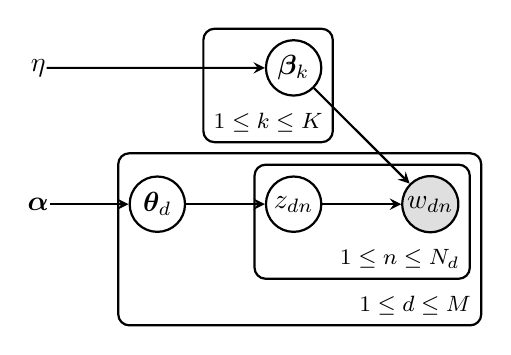
\begin{tikzpicture}[->, >=stealth, thick, scale=3.0]

    % Nodes

    \node[obs]                   (w)      {$w_{dn}$} ; %
    \node[latent, left=of w]    (z)      {$z_{dn}$} ; %
    \node[latent, left=of z]    (theta)  {$\bm{\theta}_d$}; %
    \node[const, left=of theta] (alpha) {$\bm{\alpha}$};

    \edge {z} {w}
    \edge {theta} {z}
    \edge {alpha} {theta}

    % More nodes
    \node[latent, above=of z] (beta)  {$\bm{\beta}_k$}; %
    \node[const]  (eta) at (alpha |- beta) {$\eta$}; %

    \edge {beta} {w}
    \edge {eta} {beta}

    \plate {plate1} { %
        (w)
        (z)
    } {$1 \leq n \leq N_d$}; %
    \plate {} { %
        (plate1) %
        (theta)
    } {$1 \leq d \leq M$} ; %
    \plate[align=left] {} { %
        (beta)
    } {$1 \leq k \leq K$} ; %

\end{tikzpicture}
\end{center}

\end{document}
